\styledchapter{Markets and Auctions}
\section{Independent Private Values}

Consider now $m$ homogeneous units of an indivisible good available (an inelastic supply). There are $N$ bidders, each with single-unit demand.
Let $v_i \in \left[ 0,1 \right]$ be $i$'s value for one unit of the good, where $v_i$ has density $f_i$. 

If $i$'s value (for one unit) is $v_i$, her demand function is \[
	Q(p) = \begin{cases}
		0, p > v_i \\
		1, p \le v_i
	\end{cases}
.\] 
Let $X_1 \ge \cdots X_N$ be the order statistics of $V_1,\ldots,V_N$.
If
\[
	X_1 = x_1 > X_2 = x_2 > \cdots > X_N = x_n,
\]
then the market demand function is
\[
	Q(p) = \sum\limits_{i=1}^{n} \mathds{1}_{p \le X_i}
.\] The market-clearing price is any price $p \in (x_{m+1}, x_{(m)}]$.
Note that bidders $m$ and $m+1$ may have some incentive to not report their values truthfully.

Let $b_i$ denote the ``height'' of bidder $i$'s submitted one-step demand function; i.e., the price at which she switches from wanting to buy the object vs. not. We will call $b_i$ a bid.

Let $B_{(1)} \ge B_{(2)} \ge \cdots \ge B_{(N)}$ be the order statistics of bids $b_1,b_2,\ldots,b_N$.
The range of market-clearing prices is $p \in (B_{(m+1)}, B_{(m)}]$.

	We wan to set a rule for the market-clearing price. We shall always choose the highest market-clearing price: namely, $B_{(m+1)}$, which is the $(m+1)$st-highest bid. With this rule, the bidders submit a (sealed) bid.\boxednote{If $m=1$, this is a second-price auction.}

	\begin{proposition}	It is a dominant strategy to bid your value.\boxednote{If instead $p = B_{(m)}$, a bidder can affect the clearing price directly, so truthful bidding is no longer dominant.}
	\end{proposition}
\begin{proof}
	We notate $B_{(k)}^{-i}$ as the $k$th highest bid of the bidders other than $i$. If bidder $i$ wins a good, she pays $B_{(m)}^{-i}$. You want to win when $v_i > B_{(m)}^{-i}$ and lose when $v_i < B_{(m)}^{-i}$. Since your bid does not affect $B_{(m)}^{-i}$, then bidder $i$ cannot affect the price, then we can accomplish this by bidding $b_i = v_i$.
\end{proof}

\begin{remark}	In this equilibrium, the outcome is efficient.
\end{remark}

\section{Interdependent Values, Affiliated Private Information}
Return to the general symmetric interdependent-values model with values $V_1,\ldots,V_n$ and signals $S_1,\ldots,S_n$.
Now consider $m\ge 1$ homogeneous units of a good for sale with at most single-unit demand.
Consider an $(m+1)$st price auction.
Let $b_{N,m}^{*}(s)$ be a strictly increasing symmetric equilibrium bidding function.

Fix bidder $i$ (WLOG consider $i=1$) and let $y_1 > y_2 > \cdots > y_{N-1}$ represent the signals of the other bidders. Then if bidder $i$ wins the good, she pays $b_{N,m}^*(y_m)$. When her signal is $s$, the good is worth $\E\left[V_1 \mid S_1 - s, Y_m = y_m\right]$.

\begin{figure}[htpb]
	\centering
	\caption{Optimal bidding function against expected value of good.}
	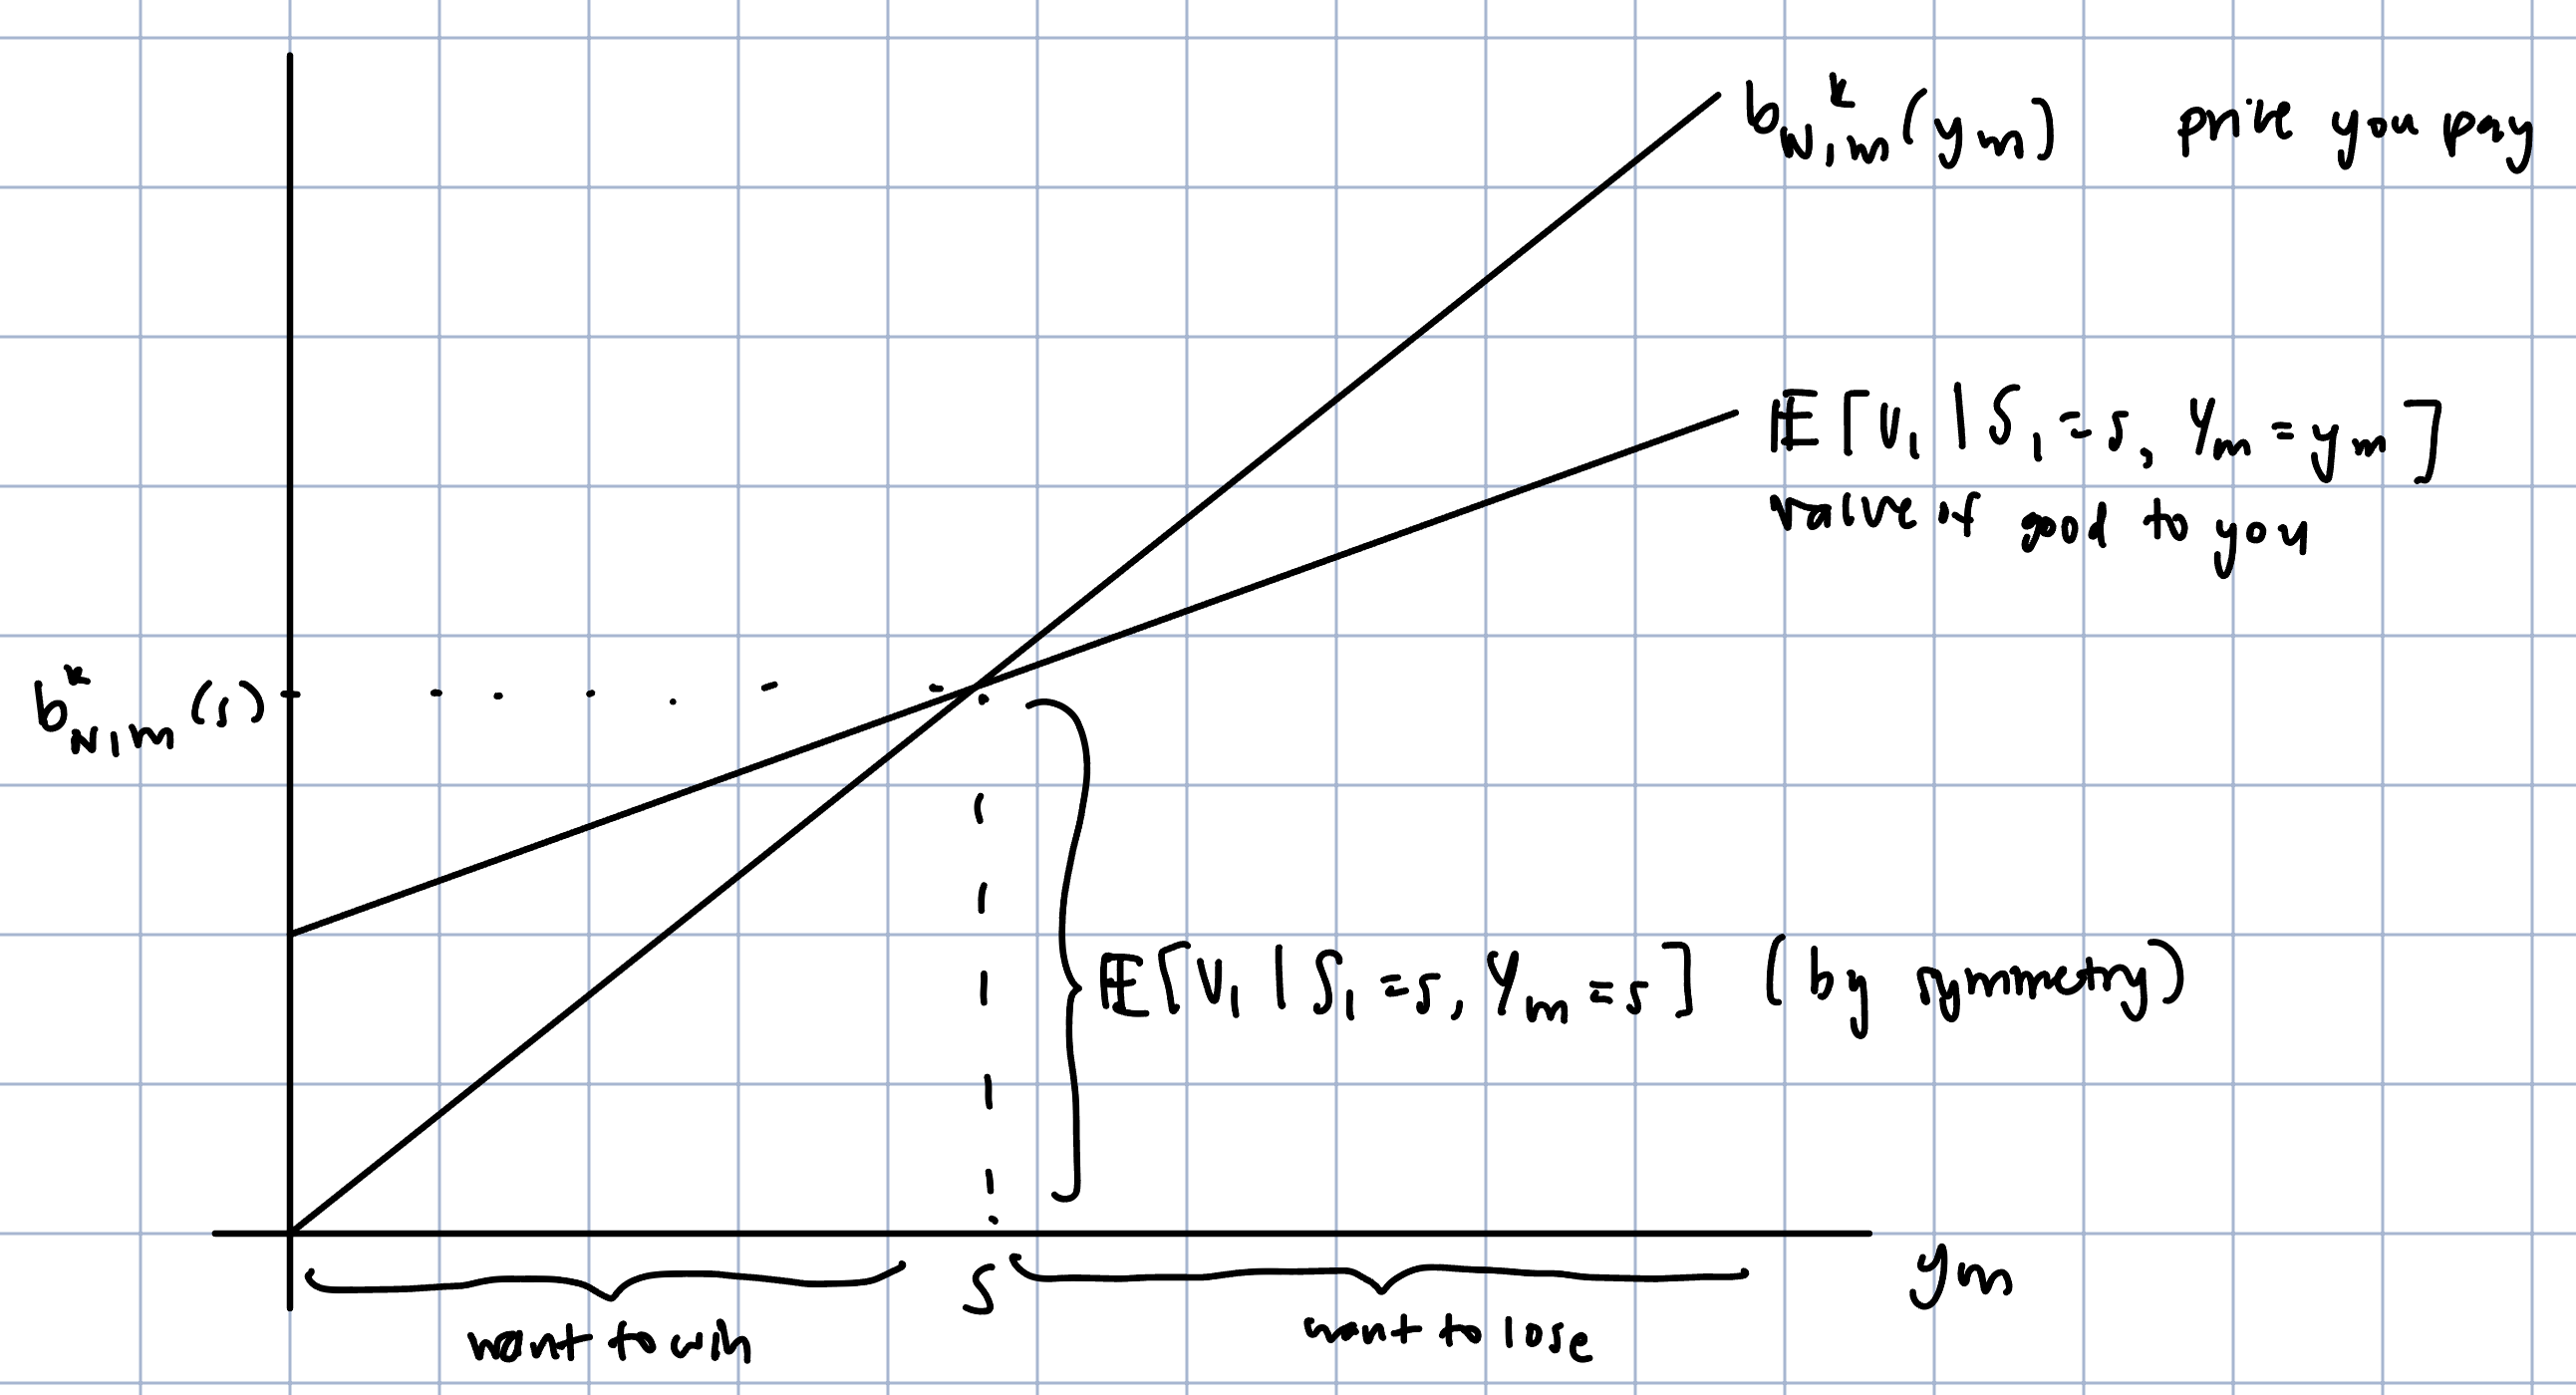
\includegraphics[width=0.78\textwidth]{images/2-19-1}
\end{figure}
Considering the picture, the optimal bidding function is \[
	b_{N,m}^*(s) = \E\left[V_1 \mid S_1 = s, Y_m = s\right] 
.\] 

When does a market price effectively aggregate and reflect private information? If the market is sufficiently large (with the intention of using the LLN), will the market price reflect the true value\footnote{Presumed to be a common value\, as in stocks, treasury bonds, IPOs, etc.} of the good?
We will specialize our model so that $V_1= \cdots = V_n = V$ and that for any given value $v \in [0,1]$, each bidder receives an independent signal drawn from $\operatorname{Uni}(0,v)$.\footnote{The distribution need not be uniform. We just require that $\frac{f\left( \overline{s}\mid v \right)	}{f(s\mid v)}$ is increasing in $v$ for $\overline{s} > s$. Equivalently, we can require that for $v_2 > v_1$, $\frac{f(s \mid v_2)}{f(s \mid v_1)}$ is increasing in $s$.} Lastly, suppose that $v$ is drawn according to the density $g(v)$ with support $[0,1]$. 

Suppose $N,m \to \infty$ such that $\frac{m}{N} \to \alpha \in (0,1)$. Since $S \sim \operatorname{Uni}(0,v)$, writing $X_1 \ge X_2 \ge \cdots \ge X_N$ as the order statistics of the signals $S_1,\ldots,S_N$, we expect \[
	X_{m+1} \to (1-\alpha)v
.\] For any bidder whose signal is $s$, \[
	b_{N,m}^{*}(s) = \E\left[V_1 \mid S_1 = s, Y_m = s\right]  \approx \E\left[V_1 \mid X_{m+1} = s\right] 
,\] so as $N,m \to \infty $ where $\frac{m}{N} \to \alpha \in (0,1)$, we have that \[
	\frac{X_{m+1}}{1-\alpha} \to v
.\] Hence, for large $N,m$, \[
	b_{N,m}^*(s) \approx \frac{s}{1-\alpha}
.\]

This implies that the price when there are $N$ bidders and $m$ units of the good is \[
	p_{N,m} = b_{n,m}^*(X_{m+1}) \approx \frac{X_{m+1}}{1-\alpha}\to \frac{(1-\alpha)v}{1-\alpha} = v
.\] 

\section{Multi-Unit Demand}
Suppose we have $m$ homogeneous units of the good for sale, $N$ bidders, and private values for each bidder $i$ of $v_i = \left( v_{i,1},\ldots,v_{i,m} \right)$ such that $v_{i, 1} \ge v_{i, 2}\ge \cdots \ge v_{i,m}$; in other words, we have demand decreasing in the number of goods bidder $i$ ends up with. We take $v_1,\ldots,v_N \in [0,1]^m$ drawn independently from $\{f_i(v_i)\}$. Each bidder $i$ will submit $m$ bids $b_i = \left( b_{i,1},\ldots,b_{i,m} \right)$.

What are the analogues of the FPA, SPA, and English auctions? Are there auctions that allocate the $m$ units efficiently?\boxednote{By efficiently, we mean that after an efficient auction, no pair of bidders would want to buy/sell some unit of the good after the conclusion of the auction. In other words, all $v_{i,k}$ associated with the $k$th unit allocated to bidder $i$ must be higher than all $v_{j,l}$ for when bidder $j$ did not receive a $l$th unit.}

Note that $v_{i,k}$ is bidder $i$'s \emph{marginal} value for a $k$th unit of the good. So, if bidder $i$ wins $k$ units and pays a total price of $p$, her utility is $v_{i,1}+ \cdots + v_{i,k}- p$.

Consider the \emph{$(m+1)$st price auction}\footnote{Also called the uniform-price auction.} as a generalization of the second price auction. 

\begin{definition}[(m+1)st-price auction (Uniform-price auction)]
	Each bidder $i$ submits $b_i = (b_{i,1},\ldots,b_{i,m})$. Without loss we can take $b_{i,1} \ge \cdots \ge b_{i,m}$. The seller orders all $N\cdot m$ bids and the $m$ highest bids win. If bidder $i$ wins $k$ units of the good, then she pays the $(m+1)$st-highest bid for each unit won, so she pays $k B_{(m+1)}$.
\end{definition}

Is the outcome always efficient in an $(m+1)$st-price auction?

\begin{example}	Let $N = m =2$ with $v_1 = (10,10)$ and $v_2 = (7,0)$. Each bidder submits two bids, and the two units of the good go to bidder $1$ in an efficient allocation.
	Under honest bidding, this is an equilibrium. But under strategic bidding, bidder $1$ could bid $(10,0)$ and be better off.

	The uniform-price auction does not lead to an efficient outcome because one can affect the $B_{(m+1)}$ bid, unlike as in the single-unit second price auction.\boxednote{Recall that in the single-unit SPA, if a bidder is the one who sets the price, then she does not win the good.} A bidder with high values for multiple units may strategically bid low on later units to still win (some) units but pay a lower price for them.
\end{example}

What if we consider a \emph{sequential second-price auction}, in which one good is auctioned off at a time? 
In the previous example, honest bidding is an equilibrium, but in strategic bidding, bidder $1$ could first bid $0$, then $10$, to increase her utility.

Consider elettering the goods $A,B,\ldots$ and run English auctions for the goods with separate price clocks. Each price clock will increase until demand for the good is $1$. With the same example as before, honest bidding is efficient, while strategic bidding is not. This is because bidder $1$ could commit to only bidding on unit $A$. Then bidder $2$ gets unit $B$ for price $0$, and bidder $1$ gets unit $A$ for price $0$.\boxednote{The prices are $0$ and not some small $\epsilon$ (or $1$ if we have discrete prices) as long as the bidders start the bidding on different goods.}

Let us consider the \emph{discriminatory auction}.
Suppose each bidder submits $b_i - \left( b_{i,1},\ldots,b_{i,m} \right)$ and the highest $m$ bids win, where winners pay their bids on each unit won. If $i$ wins $k$ units, then \[
	u_i - v_{i,1} + \cdots + v_{i,k} - \left( b_{i,1} + \cdots + b_{i,k} \right)
.\] 
Suppose $N=m=2$ and let $(\hat{b}_1,\hat{b}_2)$ denote the equilibrium bidding strategy for the discriminatory auction in which $f_i  =f$ for all $i$. Here, $\hat{b}_k (v_{i,1},v_{i,2})$ is the bid on a $k$th unit submitted by $i$ when $v_i= (v_{i,1},v_{i,2})$.

Assuming that $\hat{b}_k$ is strictly increasing in $v_{i,1}$ and $v_{i,2}$.

What would this bidding function look like?
Laboriously, we find that when $v_{i ,1} \approx v_{i, 2}$, because $i$'s bid for a first unit is against the lower bid distribution of $\hat{b}_2 \left( v_{j,1}, v_{j,2} \right)$ than $i$'s bid for a second unit against the higher distribution $\hat{b}_1 \left( v_{j,1},v_{j,2}\right)$ is, we reason that \emph{ideally} $i$ would want $b_{i,1} \le b_{i,2}$.  

\boxednote{Maybe it would be a good idea to characterize exactly when it is not efficient.}
This auction is not efficient with positive probability. 

\section{Vickrey's Auction}
We want an auction that allocates the $m$ units to the bidders with the highest $m$ vlaues. If we can get the bidders to be honestly such that \[
	b_i = \left( v_{i,1},\ldots,v_{i,m} \right), \quad \forall\ i
,\] then allocating the units to the $m$ highest bids will be efficient. So, let's focus on sealed-bid auctions that allocated units to the $m$ highest bids. The remaining task is to determine a payment structure that is incentive-compatible.\boxednote{Is there an auction design that is not incentive-compatible but still has bids increasing in values, so it is efficient? (Besides some case where you pay $\alpha$ times the bid we derive, so you bid $\frac{v}{\alpha}$.)}
We will assume for (and verify later that such a design is possible) that one will only pay if she wins some units.

Suppose $N=m=2$, and suppose bidders $2$ bids $b_2 = \left( b_{2,1}, b_{2,2} \right)$, with $b_{2,1} > b_{2,2}$. Can we define a payment rule for bidder $1$ that makes him win when he wants ot win and lose when he wants to lose when he bids honestly?

Let $p_{1,1}$ and $p_{1,2}$ be the prices bidder $1$ would pay for the first and second unit. If bidder bids honestly, he wins at least one unit iff $v_{1,1} > b_{1,1} > b_{2,2}$ and wins a second unit iff $v_{1,2} = b_{1,2} > b_{2,1}$. He wants to win a first unit when $v_{1,1} > p_{1,1}$ and a second unit when $v_{1,2} > p_{1,2}$.
Then we can set $p_{1,1} = b_{2,2}$ so the first-unit condition is satisfied, and set $p_{1,2} = b_{2,1}$ so the second-unit condition is satisfied.\boxednote{Note that bidder $i$ cannot influence the prices she pays, and over/underbidding can only result in winning a unit when she doesn't want to/wants to win.}

We write this generically as the pricing rule\boxednote{Under this pricing rule, bidder $i$ only pays for units she receives, as we assumed.} \[
	p_{i 1} = b_{j 2}, \quad p_{i 2} = b_{j 1}, i \ne j
.\] 

Now consider $N=2$ and $m$ units.
If bidder $1$ bids honestly, so
\[
	b_1 = v_1 = \left( v_{1,1},\ldots,v_{1,m} \right),
\]
and bidder $2$'s bids are fixed at $b_2 = \left( b_{2,1},\ldots,b_{2,m} \right)$, then
\begin{itemize}
	\item Bidder $1$ wins at least one good if $b_{1,1} = v_{1,1} < b_{2,m}$,
	\item Bidder $1$ wins at least two goods if $b_{1,2} = v_{1,2} < b_{2,m-1}$,
	\item and so on.
\end{itemize}
Hence, $v_{1,1}$ competes against $b_{2,m}$, $v_{1,2}$ competes aaginst $b_{2,m-1}$, $v_{1,3}$ competes against $b_{2,m-2}$, and so long.

Analogously,
\begin{itemize}
	\item Bidder $1$ wants to win at least one good if $v_{1,1} > p_{1,1}$,
	\item Bidder $1$ wants to win at least two goods iff $v_{1,2} > p_{1,2}$,
	\item and so on.
\end{itemize}

Therefore, we should put \[
	p_{1,k} = b_{2m - k +1}
.\] 

\begin{remark}
	We can check incentive-compatibility by asking whether honest bidding admits any unilateral profitable deviation.
	Suppose $b_i = \left( v_{i_1},\ldots,v_{i,m} \right)$ and bidder $i$ wants to win $k$ units, while bidder $j$ bids $b_j = \left( b_{j,1},\ldots,b_{j,m} \right)$.
	Then $v_{i,1},v_{i,2},\ldots,v_{i,k}$ and $b_{j,1},b_{j,2},\ldots,b_{j,m-k}$ are the $m$ highest bids.

	Would bidder $i$ have liked to submit a different bid vector and win a different number of units? For a $k+1$st good, bidding $i$ must pay $b_{j,m-k}$, which by being in the highest $m$ bids, is larger than $v_{i,k+1}$, which is not in the highest $m$ bids. The same applies to the values vs. prices for the $k+2$nd good and so one. Similarly, the $k$th unit that bidder $i$ won has value $v_{i,k} > b_{j,m-k} = p_{i,k}$, and so on for the $k-1$st and earlier units. 

	We note that bidder $i$, having won $k$ units, pays the sum of the $k$ losing bids of his opponent. The same pricing rule applies to the second-price auction, so this generalizes the SPA.
\end{remark}

Now suppose we have $N$ bidders and $m$ units. 
\begin{definition}[Vickrey auction]
	Suppose $N$ bidders submit $m$ sealed bids and the $m$ highest bids win. If a bidder wins $k$ units, then she pays the sum of the $k$ highest losing bids of her opponents.
\end{definition}

\begin{theorem}[Efficiency of Vickrey Auction]
	Bidding honestly is a dominant strategy in a Vickey auction. Thus, the outcome of rational bidding is efficient.
\end{theorem}
\begin{proof}
	If bidder $i$ bids truthfully with $b_i = \left( v_{i,1},\ldots,v_{i,m} \right)$ and bidders $j \ne i$ bid $\left( b_{j,1},\ldots,b_{j,m} \right)$.
	Let $B^{-i}_{(k)}$ be the $k$th highest bid of the others. Put the price $i$ pays for a $k$th unit be $p_{i,k}$. Bidder $i$ wins a first unit iff $v_{i,1} > B^{-i}_{(m)}$, a second unit iff $v_{i,2} > B^{-i}_{(m-1)}$, and so on.

	The reasoning for the proof is similar to the $N = 2$ case we already saw.
\end{proof}

\section{Efficiency and Interdependent Values, Multiple Units and Multi-Unit Demand in the Vickrey Auction}
We specialize to $N=2$ and $m$ units. Each bidder $i=1,2$ receives a signal $s_i$. Let $v_{i,k}\left( s_1,s_2 \right)$ denote $i$'s value for a $k$th unit when the signals are $s_1,s_2 \in [0,\infty)$. For example, we may have \[
	v_{i,k}(s_1,s_2) = \E\left[V_{i,k} \mid S_1 = s_1,S_2 = s_2\right] 
,\] 
but we will make assumptions on the values of marginal goods $v_{i,k}(s_1,s_2)$ directly.

\begin{assumption}	We assume for every $s_1,s_2$ and $k,l, i \ne j$, 
	\begin{enumerate}[label=(\roman*)]
		\item $v_{i,k}(s_1,s_2) \ge v_{i, k+1}(s_1,s_2) \ge 0$ 
		\item $v_{i,k}(s_1,s_2)$ is strictly increasing in $s_i$ and nondecreasing in $s_j$
		\item The partials satisfy \[
			\frac{\partial v_{1,k}(s_1,s_2)}{\partial s_1} \ge \frac{\partial v_{2,l}(s_1,s_2)}{\partial s_1}, \quad \frac{\partial v_{1,k} (S_1,s_2)}{\partial s_2} \le \frac{\partial v_{2,l} (s_1,s_2)}{\partial s_2}
		.\] 
		\item There exist unique $\alpha,\beta$ such that \[
				v_{i,k}(s_1,\alpha) = v_{2,l}(s_1,\alpha), \quad v_{1,k}(\beta,s_2) = v_{2,l}(\beta,s_2)
		.\] This assumption is stronger than what's needed but simplifies things.
	\end{enumerate}
\end{assumption}

Let $\hat{b}_i(s_i) = \left( \hat{b}_{i,i}(s_i),\ldots,\hat{b}_{i,m}(s_i) \right)$ for $i \in \left\{1,2\right\}$ be the equilibrium bidding vectors when the bidders have signals $s_1$ and $s_2$. Assume all $\hat{b}_{i,k}(s_i)$ are increasing in $s_i$.

As we know $\hat{b}_{1,k}(s_1)$ competes against $\hat{b}_{2,m-k+1}(s_2)$ and vice versa. Also, $\hat{b}_{2,m-k+1}(s_2)$ is the marginal price that bidder 1 pays for the $k$th unit she wins and $\hat{b}_{1,k}(s_1)$ is the marginal price that bidder 2 pays for his $m-k+1$st unit. Hence, bidder 1's optimal bid for a $k$th unit depends on $\hat{b}_{2,m-k+1}(s_2)$ and bidder 2's optimal bid for a $m-k+1$st unit depends on $\hat{b}_{1,k}(s_1)$. We need to derive these together, as each function appears in the other's first-order condition.

Let $s_1^{0}$ be any signal for bidder 1. We'd like to determine $\hat{b}_{1,k}(s_1^{0})$.

\begin{figure}[htpb]
	\centering
	\caption{Derivation of the paired bidding functions.}
	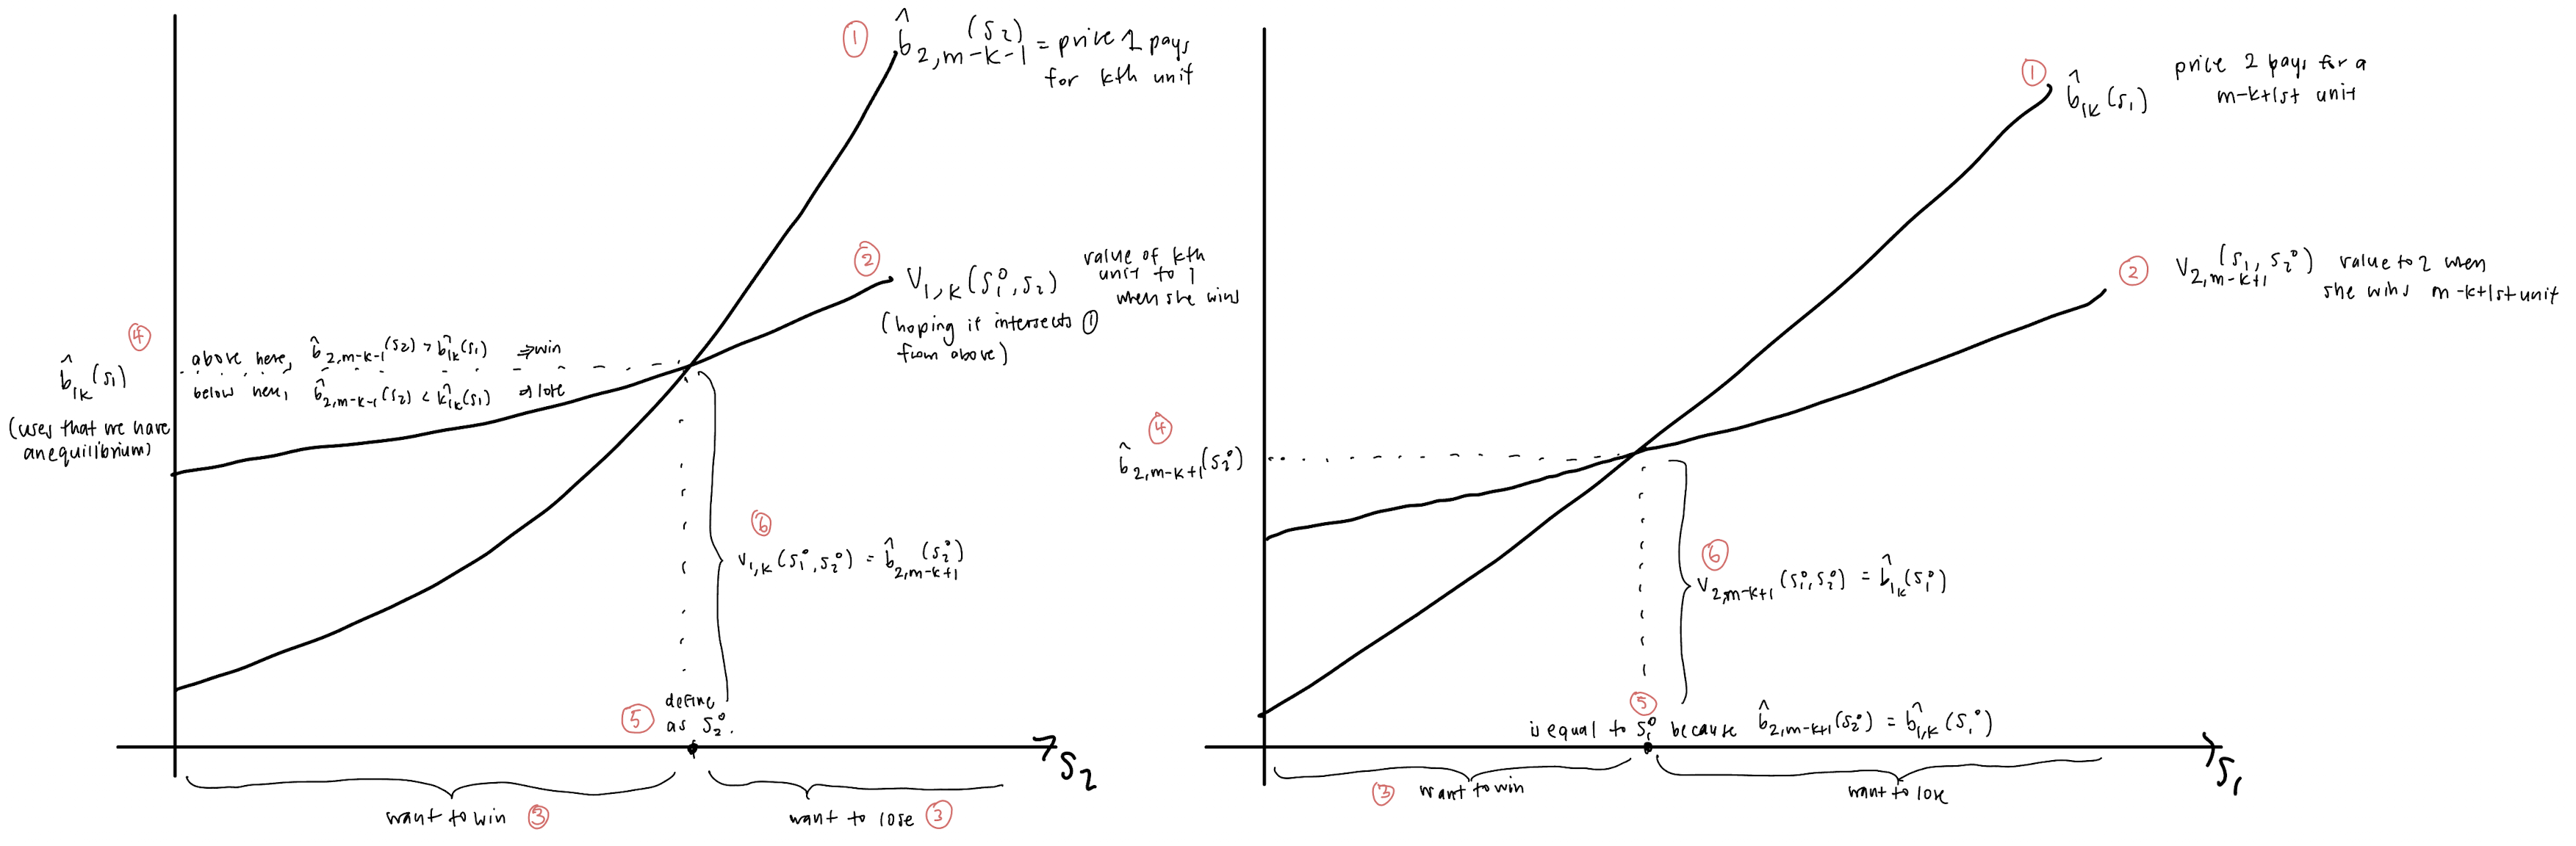
\includegraphics[width=0.78\textwidth]{images/3-3-1}
\end{figure}

The graphs each depict an equilibrium condition: at the marginal threshold $(s_1^0, s_2^0)$ where bidder 1's bid for unit $k$ exactly ties bidder 2's competing bid for unit $m-k+1$, each bidder optimally bids their true value at that threshold.
Note that from the first graph, we have the equation \[
	\hat{b}_{1,k}(s_1^{0}) = v_{1,k}(s_1^{0},s_2^{0}) = \hat{b}_{2,m-k+1}(s_2^{0})
.\]
Furthermore, from the second graph, \[
	\hat{b}_{2,m-k+1}(s_2^{0}) = v_{2,m-k+1}(s_1^{0}, s_2^{0}) = \hat{b}_{1,k}(s_1^{0})
.\]
Since both conditions hold simultaneously, combining them gives \begin{equation} \label{3-3-1}
	\hat{b}_{1,k}(s_1^{0}) = v_{1,k}(s_1^0 , s_2^0) = v_{2, m-k+1}(s_1^0, s_2^0) = \hat{b}_{2,m-k+1}(s_2^{0})
.\end{equation} 
Our assumption (iv)	 allows us to define the bidding functions. To see why, consider a unit $k$, signal $s$. By (iv), there is a unique signal for bidding 2 such that \[
	v_{1,k}(s_1,\alpha) = v_{2,m-k+1}(s_1,\alpha)
	.\] By\boxednote{The $\alpha$ corresponds to $s_2^0$ when $s = s_1^0$.} equation (\ref{3-3-1}), we should define for every good $k$ and signal $s$ \[
	\hat{b}_{1,k}(s_1) = v_{1,k}(s_1,\alpha)
.\] Similarly, we can find for any $k$ and $s_1$ the unique $\beta$ such that \[
	v_{2,k}(\beta,s_2) = v_{1,m-k+1}(\beta,s_2)
\] and set \[
	\hat{b}_{2,k}(s_2) = v_{2,k}(\beta,s_2)
.\] 

We now have candidate equilibrium bidding functions. 
Note that when $\hat{b}_{1,k}(s_1) = v_{1,k}(s_1,\alpha)$, then $\alpha$ depends on $k$ and $s_1$. By our assumptions, we see that $\alpha(s_1,k)$ is increasing in $s_1$ and decreasing in $k$: as $s_1$ increases, assumption~(iii) implies $v_{1,k}$ grows faster than $v_{2,m-k+1}$, pushing the crossing $\alpha$ upward; as $k$ increases, $v_{1,k}$ falls (by~(i)) while $v_{2,m-k+1}$ rises, pushing $\alpha$ downward. Similarly, $\beta(s_2,k)$ is increasing in $s_2$ and decreasing in $k$.
Hence, $\hat{b}_{i,k}(s_i)$ is strictly increasing in $s_i$. Nice! Furthermore, \[
	\hat{b}_{i,1}(s_i) \ge \cdots \ge \hat{b}_{i,m}(s_i)
.\] 

\begin{proposition}[Efficiency of the equilibrium bidding functions]
	The candidate bidding functions $\hat{b}_{1,k}$ and $\hat{b}_{2,k}$ defined above yield an efficient allocation for every signal realization.
\end{proposition}
\begin{proof}
	We must show that these functions yield an equilibrium and an efficient outcome. We show the latter first.
	Let $s_1^0, s_2^0$ be a pair of signals such that it would be efficient for bidder 1 to receive $k$ units and bidder 2 to receive $m-k$ units. Notate $s^0 := \left( s_1^0, s_2^0 \right)$. Thinking \marginimage[Partition of signals.]{3-3-2} or by referring to the image in the margin, we know
	\begin{align}
		v_{1,k}(s_1^0,s_2^0) &> v_{2,m-k+1}(s_1^0,s_2^0) \label{3-3-4}\\
		v_{2,m-k}(s_1^0,s_2^0) &> v_{1,k+1}(s_1^0, s_2^0) \label{3-3-5}
	.\end{align}
	Equation~(\ref{3-3-4}) says bidder 1's marginal value for the $k$th unit exceeds bidder 2's value for the $(m-k+1)$th, so the $k$th unit belongs to bidder 1 in an efficient allocation; equation~(\ref{3-3-5}) is the symmetric statement for bidder 2's $(m-k)$th unit.

	We must show that if the two bidders use their $\hat{b}$ bidding functions, then when their signals are $s_1^0$ and $s_2^0$, bidder 1 wins exactly $k$ units.
Since
\[
	\hat{b}_{1,k}(s_1^0) = v_{1,k}(s_1^0, \alpha) = v_{2,m-k+1}(s_1^0,\alpha),
\]
equation (\ref{3-3-4}) and assumption (iii) imply that $\alpha > s_2^0$.\boxednote{The gap \[v_{1,k}(s_1^0,s_2^0) - v_{2,m-k+1}(s_1^0,s_2^0) > 0\] by (\ref{3-3-4}), and by assumption~(iii) it is decreasing in $s_2$. So the zero of the gap, $\alpha$, must lie above $s_2^0$.}
Thus
\[
		\hat{b}_{1,k}(s_1^0) = v_{1,k}(s_1^0,\alpha) \ge v_{1,k}(s_1^0, s_2^0)
	,\] where the inequality uses $\alpha \ge s_2^0$ and that $v_{1,k}$ is nondecreasing in $s_2$ (assumption~(ii)).
	Similarly, since \[\hat{b}_{2,m-k+1}(s_2^0) = v_{2,m-k+1}(\beta,s_2^0) = v_{1,k}(\beta,s_2^0),\]
	equation (\ref{3-3-4}) and assumption (iii) give for $\beta < s_1^0$
	\begin{equation} \label{3-3-6}
		\hat{b}_{2,m-k+1}(s_2^0) = v_{2,m-k+1}(\beta,s_2^0) \le v_{2,m-k+1}(s_1^0,s_2^0)
	.\end{equation}
	Chaining these two bounds with equation~(\ref{3-3-4}) gives \[\hat{b}_{1,k}(s_1^0) \ge v_{1,k}(s^0) > v_{2,m-k+1}(s^0) \ge \hat{b}_{2,m-k+1}(s_2^0),\]
	so $\hat{b}_{1,k}(s_1^0) > \hat{b}_{2,m-k+1}(s_2^0)$: bidder 1 wins the $k$th unit.
	We symmetrically get from equation (\ref{3-3-5}) and assumption (iii) that
	\begin{equation} \label{3-3-7}
		\hat{b}_{2,m-k}(s_2^0) \ge v_{2,m-k}(s_1^0,s_2^0) > v_{1,k+1}(s_1^0,s_2^0) \ge \hat{b}_{1,k+1}(s_1^0),
	\end{equation}
	so $\hat{b}_{2,m-k}(s_2^0) > \hat{b}_{1,k+1}(s_1^0)$: bidder 1 does not win the $(k+1)$th unit.

	Equations (\ref{3-3-6}) and (\ref{3-3-7}) are exactly what determine an efficient outcome, so the outcome is efficient regardless of the signals.
\end{proof}

\begin{example}
	Consider $m=2$, where \[
		v_{1,1}(s_1,s_2) = 30s_1 + 20s_2,\quad v_{1,2}(s_1,s_2) = 20s_1 + 10s_2
	\] and \[
		v_{2,1}(s_1,s_2) = 12s_1 + 50s_2, \quad v_{2,2}(s_1,s_2) = 10s_1 + 40s_2
	.\] To find $\hat{b}_1(\cdot )$ and $\hat{b}_2(\cdot )$, we want to find $\alpha$ \footnote{We know such an $\alpha$ always exists by our assumptions, which gave us this procedure of finding the bidding functions.}such that \[
		\hat{b}_{1,1} (s_1) = v_{1,1}(s_1, \alpha) = v_{2,2}(s_1,\alpha)
	,\] i.e. solving \[
		30s_1 + 20\alpha = 10s_1 + 40\alpha
	,\] which yields $\alpha = s_1$, so $\hat{b}_{1,1}(s_1) = 50s_1$.
	We do the same for bidder 1's second unit (and bidder 2's first): find $\alpha$ such that \[
		\hat{b}_{1,2}(s_1) = v_{1,2}(s_1,\alpha) = v_{2,1}(s_1,\alpha)
	,\] i.e. solving \[
		20s_1 + 10 \alpha = 12 s_1 + 50\alpha
	,\] which yields $\alpha = \frac{1}{5}s_1$, so $\hat{b}_{1,2}(s_1) = 22s_1$.

	Symmetrically, we find $\beta$ such that \[
		\hat{b}_{2,1}(s_2) = v_{2,1}(\beta, s_2) = v_{1,2}(\beta, s_2)
	,\] i.e. \[
		12\beta + 50s_2 = 20\beta + 10s_2
	,\] so $\beta= 5s_2$ and $\hat{b}_{2,1}(s_2) = 110s_2$. Lastly, we find $\beta$ such that \[
		\hat{b}_{2,2}(s_2) = v_{2,2}(\beta, s_1) = v_{1,1}(\beta, s_2)
	,\] i.e. \[
		1-\beta + 40s_2 = 30\beta + 20s_2
	.\] We find $\beta = s_2$ and $\hat{b}_{2,2}(s_2) = 50s_2$.


	If $s_1=  1$ and $s_2=2$, then \[
		\hat{b}_{1,1}(1) = 50, \ \hat{b}_{1,2}(1) = 22,\ \hat{b}_{2,1}(2) = 220,\ \hat{b}_{2,2}(2) = 100
	.\] So bidder $2$ bids 22 for the first unit and 50 for the second unit, totalling 72. Bidder 2 would not like to give up her second unit nor her second unit and her first, and bidder 1 would not like to win a first unit, nor a first unit and a second unit, so the outcome is an equilibrium. It is also efficient.
\end{example}
